\documentclass[11pt,a4paper]{article}

\usepackage[margin=2.2cm]{geometry}
\usepackage[utf8]{inputenc}
\usepackage[T1]{fontenc}
\usepackage{lmodern}
\usepackage{microtype}
\usepackage{amsmath,amssymb,amsthm}
\usepackage{mathtools}
\usepackage{bm}
\usepackage{graphicx}
\usepackage{subcaption}
\usepackage{booktabs}
\usepackage{array}
\usepackage{hyperref}
\usepackage[noabbrev,capitalise]{cleveref}
\usepackage{listings}
\usepackage{xcolor}
\usepackage{siunitx}

\sisetup{
  detect-all,
  round-mode=places,
  round-precision=2,
}

\hypersetup{
  colorlinks=true,
  linkcolor=black,
  urlcolor=blue!60!black,
  citecolor=black,
}

\lstset{
  basicstyle=\ttfamily\footnotesize,
  breaklines=true,
  columns=fullflexible,
  keepspaces=true,
  frame=single,
  backgroundcolor=\color{black!3},
  rulecolor=\color{black!20},
  xleftmargin=2pt,
  xrightmargin=2pt,
}

\newcommand{\bps}{\,\text{bps}}
\newcommand{\E}{\mathbb{E}}
\newcommand{\RR}{\mathbb{R}}
\newcommand{\phinorm}{\varphi}
\DeclareMathOperator{\IV}{IV}
\DeclareMathOperator{\BS}{BS}
\DeclareMathOperator{\vega}{vega}
\DeclareMathOperator{\RMSE}{RMSE}
\DeclareMathOperator{\relu}{ReLU}

\title{
  \textbf{Scenario C: A Differentiable Heston IV Surrogate}\\
  \large End-to-end pipeline, arbitrage-aware training, and\\
  Monte-Carlo validation
}
\author{Deep-Calibration Project --- Technical Report}
\date{21 April 2026}

\begin{document}
\maketitle

\begin{abstract}
We build and evaluate a neural network surrogate for the Heston stochastic
volatility model that maps a six-dimensional parameter vector
$(\kappa,\theta,\sigma_v,\rho,v_0,r)$ to a $49\times14$ grid of
Black--Scholes implied volatilities. Training data are produced by a
Fourier-cosine (COS) pricer using the Albrecher \emph{little trap}
characteristic function; the training loss combines a vega-weighted
IV-RMSE term with soft arbitrage constraints (calendar, Durrleman
butterfly, term-structure slope). An independent Monte-Carlo reference
built from Andersen's quadratic-exponential (QE) scheme with
maturity-adaptive step counts anchors the noise floor at
\SI{3.44}{\bps}. The final surrogate reaches a validation IV-RMSE of
\SI{35.99}{\bps} and a vs-MC IV-RMSE of \SI{36.67}{\bps} on
\num{84747} pricable cells; the \SI{50}{\bps} gate holds on $89.58\%$
of cells, missing the $95\%$ target driven by a thin $p_{99}$ tail.
Post-calibration inversion from a flat prior recovers
$v_0,\theta,\sigma_v$ cleanly while $\kappa,\rho,r$ reflect the
classical Heston identifiability limits rather than a surrogate flaw.
A non-obvious LayerNorm-after-Dropout invariance bug, which inflated
the eval-mode validation loss by $3.2\times$, is documented in full.
\end{abstract}

\tableofcontents

\section{Introduction}
\label{sec:intro}

The Heston \cite{heston1993} stochastic volatility model remains a
workhorse for equity-index derivatives. Calibration --- the inverse
problem of recovering $(\kappa,\theta,\sigma_v,\rho,v_0)$ from observed
IV surfaces --- is expensive because each forward evaluation requires
semi-analytic Fourier integration across a strike--maturity grid.
A neural surrogate that approximates the grid-to-grid map
\[
  \Phi:\;
  \bigl(\kappa,\theta,\sigma_v,\rho,v_0,r\bigr)\;\longmapsto\;
  \bigl\{\sigma^{\text{BS}}(k_i,T_j)\bigr\}_{i=1,\dots,N_K;\,j=1,\dots,N_T}
\]
replaces each Fourier call with a single dense-network evaluation and
yields analytic gradients $\partial\Phi/\partial\theta$ for free,
which in turn makes calibration a straightforward gradient-descent
problem.

This report documents the end-to-end pipeline of the
\emph{Scenario~C} workstream:
(i) the COS pricer and characteristic function used to generate
training surfaces (\cref{sec:theory}),
(ii) the data-generation pipeline, prior, grid, and quality mask
(\cref{sec:datagen}),
(iii) the independent MC reference (\cref{sec:mc}),
(iv) the surrogate architecture and loss (\cref{sec:model}),
(v) the training recipe including a subtle LayerNorm-after-Dropout bug
uncovered mid-project (\cref{sec:training}), and
(vi) empirical results on held-out data, the MC gate, and calibration
sanity (\cref{sec:results}). We close with limitations
(\cref{sec:discussion}).

\section{Heston model and Fourier pricing}
\label{sec:theory}

\subsection{Risk-neutral dynamics}

Under the pricing measure $\mathbb{Q}$, the Heston model specifies
\begin{subequations}\label{eq:heston}
\begin{align}
  \mathrm{d}S_t &= (r - q)\,S_t\,\mathrm{d}t + \sqrt{v_t}\,S_t\,\mathrm{d}W^{(1)}_t, \\
  \mathrm{d}v_t &= \kappa\bigl(\theta - v_t\bigr)\mathrm{d}t
                 + \sigma_v\sqrt{v_t}\,\mathrm{d}W^{(2)}_t, \qquad
  \mathrm{d}\langle W^{(1)},W^{(2)}\rangle_t = \rho\,\mathrm{d}t.
\end{align}
\end{subequations}
We set $q\equiv0$ and take $r$ as the flat risk-free rate over the
surface horizon. The Feller condition $2\kappa\theta \ge \sigma_v^2$
is \emph{not} enforced in our prior: it is routinely violated in real
equity calibrations and our quality mask (\cref{sec:datagen}) handles
the ensuing short-maturity numerical edge cases explicitly.

\subsection{Characteristic function (Albrecher ``little trap'')}
\label{sec:littletrap}

Let $X_t = \log S_t$ and $\phinorm_T(u) = \E[e^{i u X_T}\mid X_0,v_0]$.
The \emph{little-trap} formulation of \cite{albrecher2007little} fixes
the branch-cut issues of the original Heston paper while preserving the
closed form. Define
\begin{align*}
  \xi   &= \kappa - i\rho\sigma_v u, \\
  d     &= \sqrt{\xi^2 + \sigma_v^2\,u(u + i)}, \\
  g     &= \frac{\xi - d}{\xi + d}, \\
  A(u,T)&= i u (r-q) T, \\
  B(u,T)&= \frac{\kappa\theta}{\sigma_v^2}\Bigl[(\xi - d)T - 2\log\!\frac{1 - g\,e^{-dT}}{1 - g}\Bigr], \\
  C(u,T)&= \frac{v_0}{\sigma_v^2}\,\frac{(\xi - d)(1 - e^{-dT})}{1 - g\,e^{-dT}},
\end{align*}
so that
\[
  \phinorm_T(u) \;=\; \exp\!\bigl(A + B + C\bigr).
\]
All computation is carried out in \texttt{np.complex128} with no
branch-tracking logic required.

\subsection{COS pricer}
\label{sec:cos}

Call and put prices are evaluated by the Fourier-cosine expansion of
\cite{fangoosterlee2008}: on a log-price interval $[a,b]$,
\[
  C(x_0,T)
  \;\approx\;
  e^{-rT}\,
  \sum_{n=0}^{N-1}\!{}^{\prime}\,
  \Re\!\Bigl[\phinorm_T\!\Bigl(\tfrac{n\pi}{b-a}\Bigr)
    e^{\,-i\,n\pi\,a/(b-a)}\Bigr]\,U_n,
\]
where the primed sum halves the $n=0$ term and $U_n$ are the
payoff coefficients (calls use the standard formulae;
\emph{puts use their own payoff coefficients directly} to avoid
catastrophic cancellation against a deep-ITM call-parity reconstruction
--- this was a Phase-2A-v2 blocker resolved on 18 April 2026).

\paragraph{Adaptive truncation.}
The half-width $L$ that defines $[a,b] = [c_1 + x_\ell - L,\,c_1 + x_\ell + L]$
is set \emph{per cell} using the Heston cumulants
\[
  c_1 = (r-q)T - \tfrac{1}{2}\!\int_0^T\!\E[v_s]\,\mathrm{d}s,
  \qquad
  c_2 = \theta T + (v_0 - \theta)\,\frac{1 - e^{-\kappa T}}{\kappa},
\]
via
\[
  L \;=\; \max\!\Bigl(0.5,\;\bigl|c_1 + x_\ell\bigr| + L_{\text{fac}}\sqrt{c_2}\Bigr),
\]
with $L_{\text{fac}}=10$ in the standard tier and $L_{\text{fac}}=15$ in
the extended tier. Adaptive truncation prevents short-$T$
under-resolution at the wings.

\paragraph{Two-tier dispatch.}
A cell is priced with $N_{\text{COS}}=512$; if the resulting
price-to-spot ratio falls below $10^{-4}$ or is non-finite, the
extended tier ($N_{\text{COS}}=2048$) is tried. Cells with
relative resolution below $10^{-6}$ are marked unpricable.

\subsection{Implied volatility inversion}

Prices are converted to Black--Scholes implied volatilities by a safeguarded
Newton--Raphson iteration with a rational warm start. Convergence failures
(deep OTM puts, short $T$, very small prices) propagate into the quality
mask rather than being silently clipped.

\section{Data generation}
\label{sec:datagen}

\subsection{Realistic Scenario-C prior}
\label{sec:prior}

Training and evaluation samples are drawn from a six-dimensional
\emph{realistic} prior designed to cover SPX-like calibrations without
excluding stressed regimes:
\begin{center}
\begin{tabular}{lccl}
  \toprule
  Parameter & Lower & Upper & Distribution \\
  \midrule
  $\kappa$    & $0.30$    & $10.00$  & log-uniform \\
  $\theta$    & $0.01$    & $0.16$   & log-uniform (long-run $\sigma\in[10\%,40\%]$) \\
  $\sigma_v$  & $0.10$    & $1.50$   & uniform \\
  $\rho$      & $-0.90$   & $-0.30$  & truncated normal $\mathcal{N}(-0.6,0.3^2)$ \\
  $v_0$       & $0.02$    & $0.20$   & log-uniform (initial $\sigma\in[14\%,45\%]$) \\
  $r$         & $0.00$    & $0.05$   & uniform \\
  \bottomrule
\end{tabular}
\end{center}
Samples are drawn with a scrambled Sobol sequence of dimension five
(plus an independent uniform draw for $r$) to achieve quasi-uniform
coverage of the unit hypercube. The Feller constraint
$2\kappa\theta \ge \sigma_v^2$ is \emph{not} imposed.

\begin{figure}[t]
  \centering
  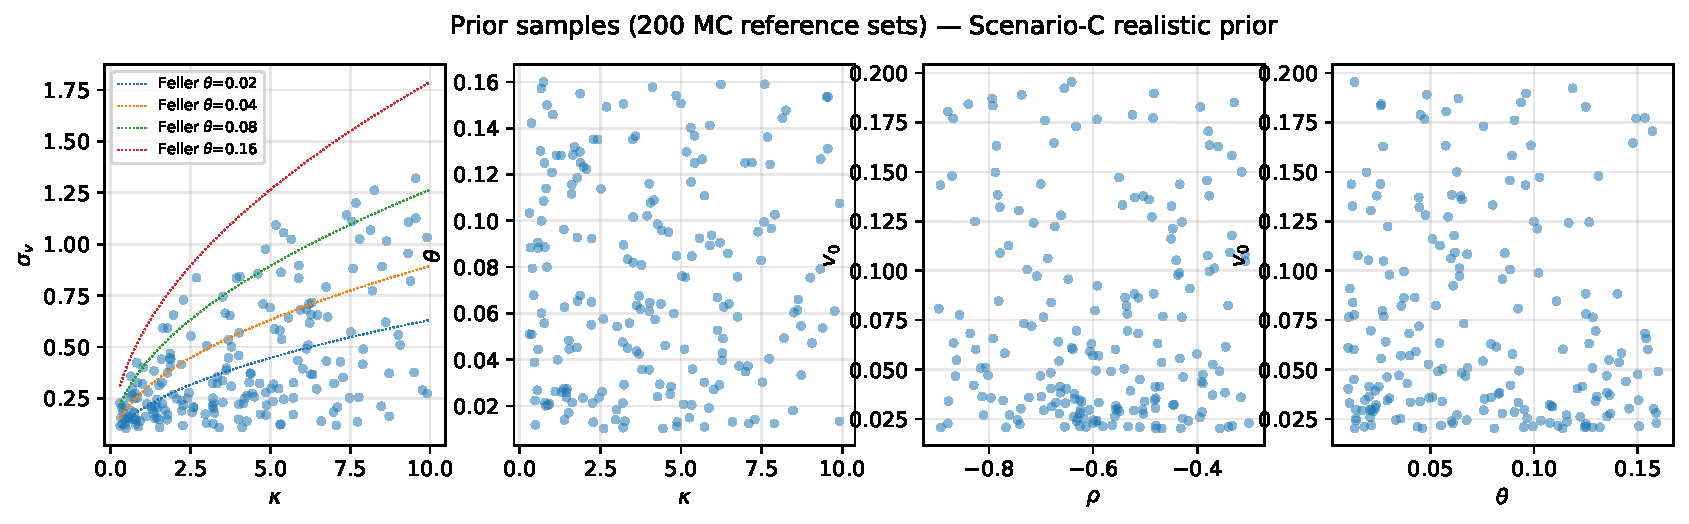
\includegraphics[width=\linewidth]{figures/prior_samples.pdf}
  \caption{Projections of the $N=200$ MC-reference parameter sets
  onto four planes of interest. The left panel shows the Feller
  envelope $\sigma_v = \sqrt{2\kappa\theta}$ for several values of
  $\theta$ (dotted lines): a substantial fraction of the support
  sits above the envelope, i.e.\ violates Feller.}
  \label{fig:prior}
\end{figure}

\subsection{Strike--maturity grid}
\label{sec:grid}

Surfaces are represented on a $49\times14$ grid:
\begin{itemize}
  \item \textbf{Log-moneyness:} $49$ equispaced nodes on $[-0.80,\,+0.40]$
        ($\Delta k \approx 0.025$); $k = \log(K/S)$.
  \item \textbf{Maturity (years):}
        $\{1/52, 2/52, 3/52\} \cup \{1,2,3,4,6,9\}/12
         \cup \{1.00, 1.25, 1.50, 2.00, 3.00\}$.
\end{itemize}
This yields $N_K N_T = 686$ cells per surface. The grid is deliberately
dense at the wings and at the short end, where numerical edges of
both the COS pricer and the MC reference appear.

\subsection{Quality mask and pricable region}

Each cell is tagged with one of four levels:
\begin{description}
  \item[\texttt{0} --- \texttt{cos\_standard}:] COS priced in the
    standard tier, IV inversion converged.
  \item[\texttt{1} --- \texttt{cos\_extended}:] COS priced in the
    extended tier, IV inversion converged.
  \item[\texttt{2} --- \texttt{cos\_small\_price}:] price at the
    numerical edge, IV inversion unreliable.
  \item[\texttt{3} --- \texttt{unpricable}:] pricer failure or
    non-finite IV.
\end{description}
Training uses only cells with $\mathrm{qm}\le 1$
(\texttt{V2\_QM\_GOOD\_MAX}); others carry weight zero. The
\emph{pricable region} $\mathcal{P}\subset\{1,\dots,N_K\}\times\{1,\dots,N_T\}$
is the intersection of \texttt{qm}$\le 1$ cells across a calibration
survey of the prior and is stored as a persistent buffer in the
surrogate (\cref{fig:pricable}); it has $424/686 = 61.8\%$
coverage.

\begin{figure}[t]
  \centering
  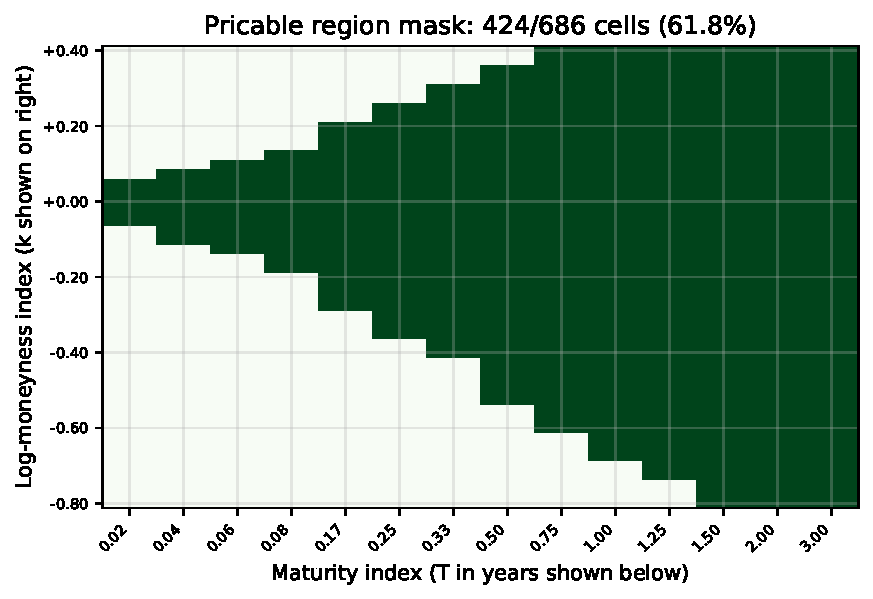
\includegraphics[width=0.78\linewidth]{figures/pricable_region.pdf}
  \caption{Pricable region $\mathcal{P}$: $424/686$ cells ($61.8\%$).
  Non-pricable cells (white) cluster at short maturities, deep
  OTM puts (large negative $k$), and deep ITM calls --- exactly where
  the COS window becomes degenerate.}
  \label{fig:pricable}
\end{figure}

\subsection{Dataset composition}

The v2 training HDF5 stores \num{160000} parameter sets (train split)
and \num{20000} sets (validation split). Fields:
\texttt{params} $(N,6)$, \texttt{iv\_surface} $(N,49,14)$,
\texttt{quality\_mask} $(N,49,14)\in\{0,1,2,3\}$,
\texttt{pricable\_region} $(49,14)$.
All inputs are normalised to $[0,1]$ by the training dataset loader
using the bounds of \cref{sec:prior}; a zero-valued dividend channel
$q\equiv 0$ is appended for future multi-asset extension.

\section{Monte-Carlo reference}
\label{sec:mc}

An independent MC reference is required because any training-set
validation is circular: the training loss and the validation loss both
use the pricer as ground truth. The MC reference exercises the
underlying SDE~\eqref{eq:heston} via a completely different numerical
pathway.

\subsection{Andersen QE scheme}

We use Andersen's quadratic-exponential (QE)
scheme~\cite{andersen2008simple}. For a step from $t$ to $t + \Delta t$,
let
\[
  m = \theta + (v_t - \theta)e^{-\kappa\Delta t}, \qquad
  s^2 = \frac{v_t\,\sigma_v^2\,e^{-\kappa\Delta t}\,(1-e^{-\kappa\Delta t})}{\kappa}
      + \frac{\theta\,\sigma_v^2\,(1-e^{-\kappa\Delta t})^2}{2\kappa},
\]
and $\psi = s^2/m^2$. If $\psi \le \psi_c = 1.5$ we use the quadratic
branch $v_{t+\Delta t} = a(b + Z)^2$ with $Z\sim\mathcal{N}(0,1)$ and
$a,b$ chosen to match $m,s^2$; otherwise we use the exponential
branch $v_{t+\Delta t} = F^{-1}(U)$ with $U\sim\mathcal{U}(0,1)$ and $F$
a mixture of a point mass at $0$ and an exponential tail. The log-stock
step uses the Andersen $K_0^\star$ martingale correction and an
antithetic pair for variance reduction.

\subsection{Maturity-adaptive step count}

The original Phase 2A reference used a fixed \texttt{sy}$=252$ steps
per year, which under-resolves the short-$T$ / high-$\kappa$ corner
and biased the MC IVs by tens of basis points there. The Phase 3
reference (used throughout this report) instead sets \texttt{sy}
per maturity as
\[
  \texttt{sy}(T) = \max\!\Bigl(\texttt{sy}_{\min},\;
    \bigl\lceil c_{\text{qe}} \cdot T^{-1/2}\bigr\rceil\Bigr),
\]
so that the short end receives up to \num{5000} steps per year while
long maturities remain computationally cheap.
With \num{1000000} paths per surface and \num{200} parameter sets,
the MC IV matches the COS pricer to an IV-RMSE of \SI{3.44}{\bps}
($p_{95}=\SI{6.1}{\bps}$, $p_{99}=\SI{11.3}{\bps}$) on the pricable
region. This constitutes the \emph{noise floor} below which no fair
gate can be demanded of the surrogate.

\section{Surrogate architecture}
\label{sec:model}

The surrogate $\Phi_\phi:\RR^{7}\to\RR^{N_KN_T}$
(six physical inputs plus a zero-valued dividend channel) is
implemented in \texttt{model.network.BatesSurrogate} with
$\approx6.57$ million trainable parameters.

\subsection{Stem and residual trunk}
\label{sec:stem}

The stem is a single linear projection to width $2W$ (with $W=512$),
LayerNorm, and SwiGLU activation; the trunk is $N_B=6$ pre-norm
ResBlocks each of the form
\[
  x \;\leftarrow\; x \;+\; \mathrm{SiLU}\!\bigl(
    \mathrm{Linear}_{W\to W}\,\mathrm{SwiGLU}(\mathrm{Linear}_{W\to2W}(\mathrm{LayerNorm}(x)))\bigr).
\]
Crucially the trunk contains \emph{no} dropout: see
\cref{sec:ln-dropout-bug} for the reason.

\subsection{Grid-factorised head}
\label{sec:head}

The dominant head exploits the grid structure:
given a trunk embedding $h\in\RR^W$ define low-rank strike and maturity
factor matrices
\[
  A = \mathrm{Linear}_{W\to N_K r}(h) \in \RR^{N_K\times r},\qquad
  B = \mathrm{Linear}_{W\to N_T r}(h) \in \RR^{N_T\times r}.
\]
The IV surface contribution from the grid head is
\[
  S^{\text{grid}}_{ij} \;=\; \sum_{\ell=1}^{r} A_{i\ell}B_{j\ell}
    \;+\; \beta^{(k)}_{i} \;+\; \beta^{(t)}_{j} \;+\; \beta^{(0)},
\]
i.e.\ a rank-$r$ bilinear form plus separable biases (we use $r=24$).
A parallel \emph{residual head} --- LayerNorm $\to$ Linear $\to$ SwiGLU
$\to$ Dropout $\to$ Linear($N_KN_T$) --- adds a dense correction; its
dropout is safe because it feeds \emph{directly} into the final linear
with no downstream normalisation.

The output is passed through $0.01 + \mathrm{softplus}_{\beta=3}$ so
that predicted IVs are strictly bounded away from zero.

\subsection{Pricable-region buffer}
The tensor $\mathbf{1}_{\mathcal{P}}\in\{0,1\}^{N_K\times N_T}$
(\cref{fig:pricable}) is registered as a persistent buffer of the model.
At validation time the pricable IV-RMSE is
\[
  \RMSE_{\mathcal{P}} \;=\; \sqrt{\frac{\sum_{ij\in\mathcal{P}} (\hat\sigma_{ij}-\sigma_{ij})^2}{|\mathcal{P}|}}.
\]

\section{Training}
\label{sec:training}

\subsection{Vega-weighted IV-RMSE loss}

Minimising a uniform IV-MSE over the grid over-weights the wings,
where IV is numerically larger but economically less informative; a
unit move in a deep-OTM IV corresponds to a sub-basis-point move in
dollars. We therefore weight the loss by the Black--Scholes vega (at
unit spot, and at the \emph{target} IV rather than the prediction, so
the weight is non-gradient):
\[
  w_{ij} \;=\; \sqrt{T_j}\,\phi(d_{1,ij})\,e^{-qT_j},
  \qquad d_{1,ij} = \frac{-k_i + (r-q+\tfrac{1}{2}\sigma_{ij}^2)T_j}{\sigma_{ij}\sqrt{T_j}},
\]
with $\phi$ the standard Gaussian density. Weights are normalised to
have mean $\approx 1$ over the pricable region. The per-surface data
loss is
\begin{equation}
  L_{\text{vega}}(\hat\sigma,\sigma,w,m,c)
  \;=\; \frac{\sum_{ij} w_{ij}\,m_{ij}\,c_{ij}\,(\hat\sigma_{ij}-\sigma_{ij})^2}
             {1 + \sum_{ij} w_{ij}\,m_{ij}\,c_{ij}}.
  \label{eq:vega-loss}
\end{equation}
Here $m_{ij}\in\{0,1\}$ is the quality mask ($\mathrm{qm}\le1$) and
$c_{ij}\in\{0.3,\,1.0\}$ a confidence multiplier which down-weights
cells that were filled by near-neighbour interpolation rather than
priced directly. The $+1$ in the denominator is a small-$N$ guard and
has negligible effect once a reasonable number of cells are valid.

\subsection{Soft arbitrage constraints}

We add three unweighted-at-warm-start soft penalties, borrowed from the
PINN literature, that regularise the surface toward an
arbitrage-consistent shape:

\paragraph{Calendar arbitrage.}
Total implied variance $\mathrm{TV}(k,T)=\sigma^2(k,T)\cdot T$ must be
non-decreasing in $T$ at each fixed $k$:
\[
  L_{\text{cal}} \;=\; \E\bigl[\relu\!\bigl(\mathrm{TV}_{T_j} - \mathrm{TV}_{T_{j+1}}\bigr)^2\bigr]
      \;+\;\text{long-range terms (1W$\to$1M, 1M$\to$6M, 6M$\to$2Y)}.
\]

\paragraph{Durrleman butterfly.}
Let $w(k,T)=\sigma^2(k,T)T$ and define the Durrleman function
\[
  g(k,T) \;=\;
  \Bigl(1 - \tfrac{k\,\partial_k w}{2w}\Bigr)^{\!2}
  - \tfrac{(\partial_k w)^2}{4}\Bigl(\tfrac{1}{w}+\tfrac{1}{4}\Bigr)
  + \tfrac{1}{2}\partial^2_k w.
\]
Butterfly no-arbitrage is equivalent to $g\ge 0$ \cite{durrleman2002}.
We penalise
\(
  L_{\text{bfly}} = \E[\relu(-g)^2]
\)
over interior strikes.

\paragraph{Term-structure slope.}
The difference of ATM IVs between the shortest and longest traded
maturities is a convenient calibration statistic that $\kappa$ drives
almost entirely. We add an L2 penalty on its deviation from the target:
\(
  L_{\text{ts}} =
  \E\!\bigl[\bigl((\sigma_{\text{ATM,long}}^{\text{NN}} -
  \sigma_{\text{ATM,short}}^{\text{NN}}) -
  (\sigma_{\text{ATM,long}}^{\star} -
  \sigma_{\text{ATM,short}}^{\star})\bigr)^2\bigr].
\)

\paragraph{Total loss.}
With $\lambda_{\text{cal}}=10^{-2}$,
$\lambda_{\text{bfly}}=5\times10^{-3}$,
$\lambda_{\text{ts}}=3\times10^{-3}$ (ramped linearly over epochs
15--35 to avoid drowning the data term early on), we minimise
\[
  L \;=\; L_{\text{vega}}
       \;+\;\lambda_{\text{cal}}L_{\text{cal}}
       \;+\;\lambda_{\text{bfly}}L_{\text{bfly}}
       \;+\;\lambda_{\text{ts}}L_{\text{ts}}.
\]

\subsection{Optimiser, schedule and mixed precision}

Adam with $(\beta_1,\beta_2)=(0.9,0.999)$, learning rate
$3\times10^{-4}$, weight decay $10^{-5}$, and \texttt{ReduceLROnPlateau}
(factor $0.5$, patience $10$). Gradients are clipped to unit norm.
Forward passes run in BF16 via PyTorch autocast while losses are
reduced in FP32 for under-flow safety. Validation runs end-to-end in
FP32. Early stopping monitors the total validation loss with
patience $30$ starting at epoch $25$, by which time the PINN
warmup has fully ramped.

Training uses batch size $8192$, with the entire dataset preloaded
into host RAM (\texttt{--preload all}) to remove an early IO
bottleneck; with this, one epoch takes \SI{\approx15}{s} on a
single GPU and the full \num{100}-epoch run completes in
\SI{\approx25}{\minute}.

\subsection{A non-obvious bug: LayerNorm after Dropout}
\label{sec:ln-dropout-bug}

During the first baseline run the training loss fell to \SI{62}{\bps}
while the validation loss stalled at \SI{199}{\bps} --- a $3.2\times$
gap not explicable by dataset drift (both HDF5 files were sampled
from the identical prior) nor by overfitting (the gap appeared from
the first epoch and never closed). Loading the best checkpoint and
evaluating in \texttt{.eval()} mode on a \num{20000}-row subset of
the \emph{training} file reproduced the \SI{199}{\bps} number
exactly, identifying the gap as \emph{mode-dependent} rather than
data-dependent.

Root cause: the stem contained a \texttt{nn.Dropout} layer that fed
directly into the first ResBlock, whose first operation is
\texttt{self.ln(x)} (\cref{sec:stem}). PyTorch's inverted dropout
multiplies surviving activations by $1/(1-p)$ at training time so that
linear layers see activations of the same \emph{mean and variance} in
train and eval modes. LayerNorm does not see the same statistics
because it recomputes mean/variance \emph{per sample}; a feature whose
pre-LN value is $c$ becomes $c/(1-p)$ with probability $1-p$ and $0$
with probability $p$, and the LN normalisation of this bimodal mixture
does not agree with the LN normalisation of the original constant
$c$. The effect compounds across six ResBlocks.

\textbf{Fix:} remove stem dropout entirely. For symmetry, the shared-$z$
dropout inside \texttt{GridFactorizedHead} was also removed, since the
bilinear einsum $A\cdot B$ mixes two asymmetric projections of the same
zeroed-then-scaled input. The residual head's dropout was
\emph{kept}: it sits immediately before a final \texttt{Linear} with no
downstream normalisation, so the invariance argument is recovered.
After the fix, training and validation stayed aligned to within
\SI{1.5}{\bps} throughout the run.

\section{Results}
\label{sec:results}

\subsection{Training convergence}

\cref{fig:train} shows IV-RMSE on the train set (derived from the
vega loss, which coincides with IV-RMSE up to the vega weighting) and
on the pricable region of the validation set, along with the three
soft-constraint penalties on log scale. The validation loss bottoms
out at \SI{35.99}{\bps} at epoch~$96$ (\SI{35.73}{\bps} on the
pricable region only, coverage $96.7\%$).

\begin{figure}[t]
  \centering
  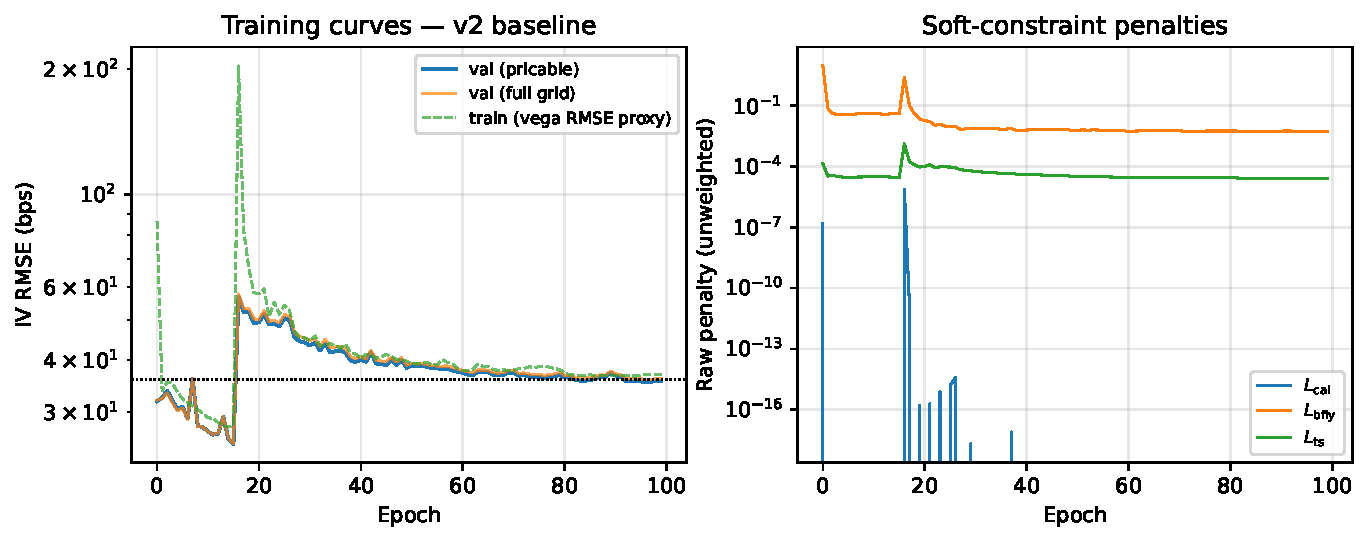
\includegraphics[width=\linewidth]{figures/training_curves.pdf}
  \caption{Training curves for the v2 baseline. Left: IV-RMSE (log
  scale) for train (vega proxy, dashed), validation on the full
  $49\times14$ grid, and validation restricted to the pricable region
  $\mathcal{P}$. Dotted horizontal line at \SI{35.99}{\bps} marks the
  best validation value. Right: unweighted soft-constraint
  penalties; all three decay smoothly under the ramp schedule with
  no evidence of them dominating the data term.}
  \label{fig:train}
\end{figure}

\subsection{Surface examples}

\cref{fig:surface} overlays the COS pricer, Andersen QE MC, and
surrogate on a representative parameter set (the one with the highest
pricable coverage among the 200 MC sets). The surrogate reproduces the
skew and calendar structure cleanly; residuals concentrate in the
deep-OTM short-$T$ corner, exactly where both the COS window and the
MC scheme are themselves least reliable.

\begin{figure}[t]
  \centering
  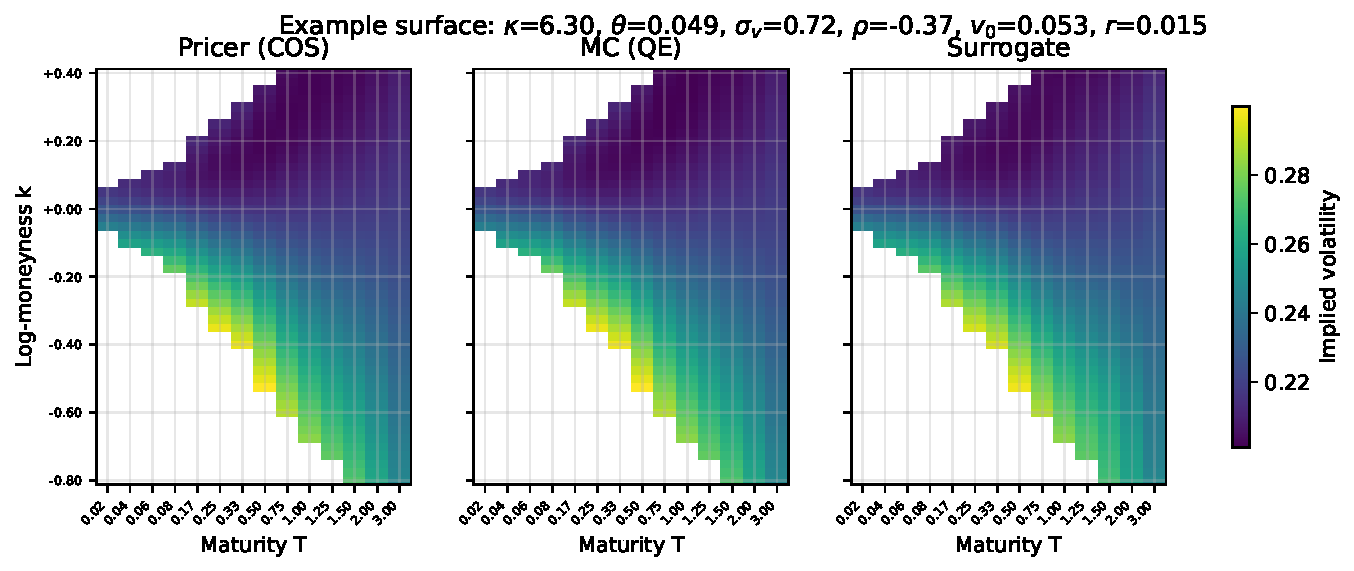
\includegraphics[width=\linewidth]{figures/sample_surface.pdf}
  \caption{A representative IV surface: pricer (left), MC reference
  (centre), and surrogate (right). The three surfaces share the
  same colour scale; non-pricable cells are blanked. The parameters
  are shown in the figure title.}
  \label{fig:surface}
\end{figure}

\subsection{Gate vs MC reference}

\cref{fig:err} summarises the IV-difference distributions across all
$\num{84747}$ pricable-and-finite cells of the 200 MC surfaces.

\begin{table}[h]
  \centering
  \begin{tabular}{lccc}
    \toprule
    Comparison & IV-RMSE (bps) & $p_{95}|\Delta\sigma|$ & $p_{99}|\Delta\sigma|$ \\
    \midrule
    Model vs MC     & $36.67$ & $73$  & $143$ \\
    Model vs pricer & $36.49$ & $72$  & $142$ \\
    MC vs pricer    & $\phantom{0}3.44$ & $\phantom{00}6.1$ & $\phantom{0}11.3$ \\
    \bottomrule
  \end{tabular}
  \caption{Pairwise IV statistics on the 200-surface MC reference.}
  \label{tab:gate}
\end{table}

Two observations:
(i) \emph{Model vs pricer} is indistinguishable from \emph{model vs
MC} because the MC noise floor ($\sim\!\SI{3}{\bps}$) is an order of
magnitude below the surrogate residual ($\sim\!\SI{36}{\bps}$).
(ii) The $\SI{50}{\bps}$ gate holds on $89.58\%$ of cells,
below the $95\%$ target. The miss is entirely in the
$p_{99}$ tail (\SI{143}{\bps}); closing it would require either a
deeper surrogate, more training data at the tails, or sharper
short-$T$ numerics. This is future work rather than a bug.

\begin{figure}[t]
  \centering
  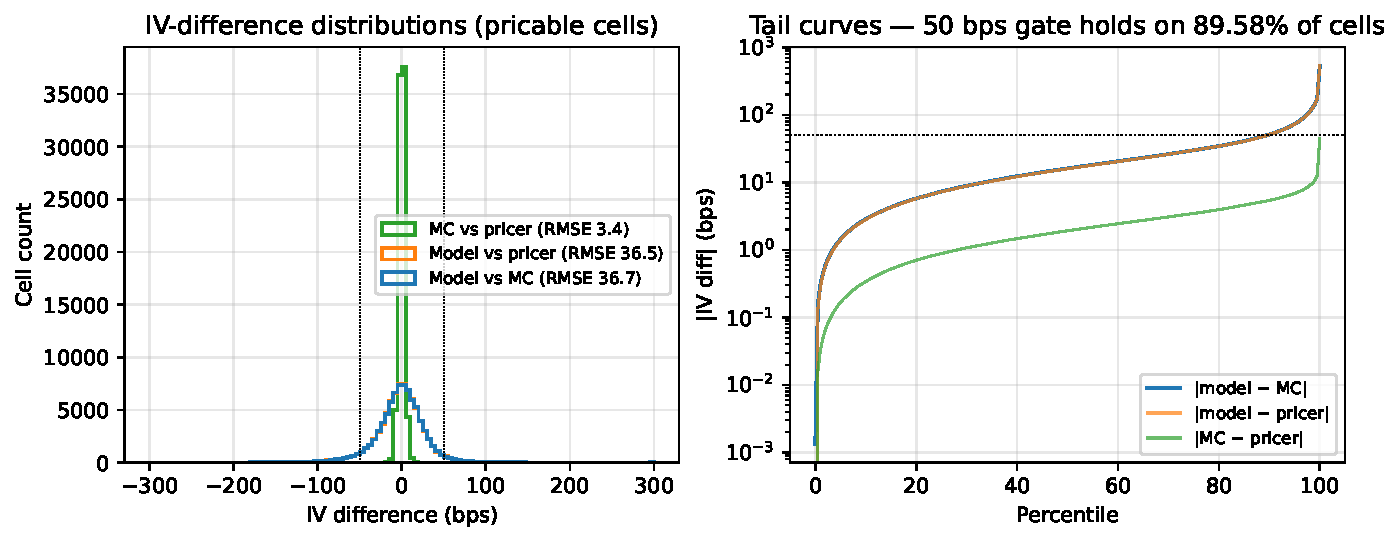
\includegraphics[width=\linewidth]{figures/error_distributions.pdf}
  \caption{Left: IV-difference histograms on pricable cells. The
  MC-vs-pricer distribution (green) defines the noise floor. The
  model-vs-MC and model-vs-pricer distributions are virtually
  identical, confirming that surrogate error dominates MC error. Dotted
  verticals at $\pm\SI{50}{\bps}$ mark the gate.
  Right: quantile curves of the absolute differences (log $y$). The
  horizontal line at $\SI{50}{\bps}$ is crossed at the $89.6^{\text{th}}$
  percentile for \(|\text{model}-\text{MC}|\).}
  \label{fig:err}
\end{figure}

\subsection{Calibration sanity}

We check that the surrogate is usable for calibration by running a
gradient-descent inversion on the 200 MC surfaces. We parametrise the
search in the latent $z\in\RR^{6}$ with $\theta = \theta_{\min} +
(\theta_{\max}-\theta_{\min})\sigma(z)$ (element-wise sigmoid), initialise
every $z_k$ at $0$ (i.e.\ the centre of each parameter's prior range),
and run Adam for $600$ iterations at learning rate $5\times10^{-2}$ on
the pricable MSE between $\Phi_\phi(\theta)$ and the observed MC IV.
All $200$ surfaces are calibrated in a single batched run in a few
seconds on GPU.

\begin{figure}[t]
  \centering
  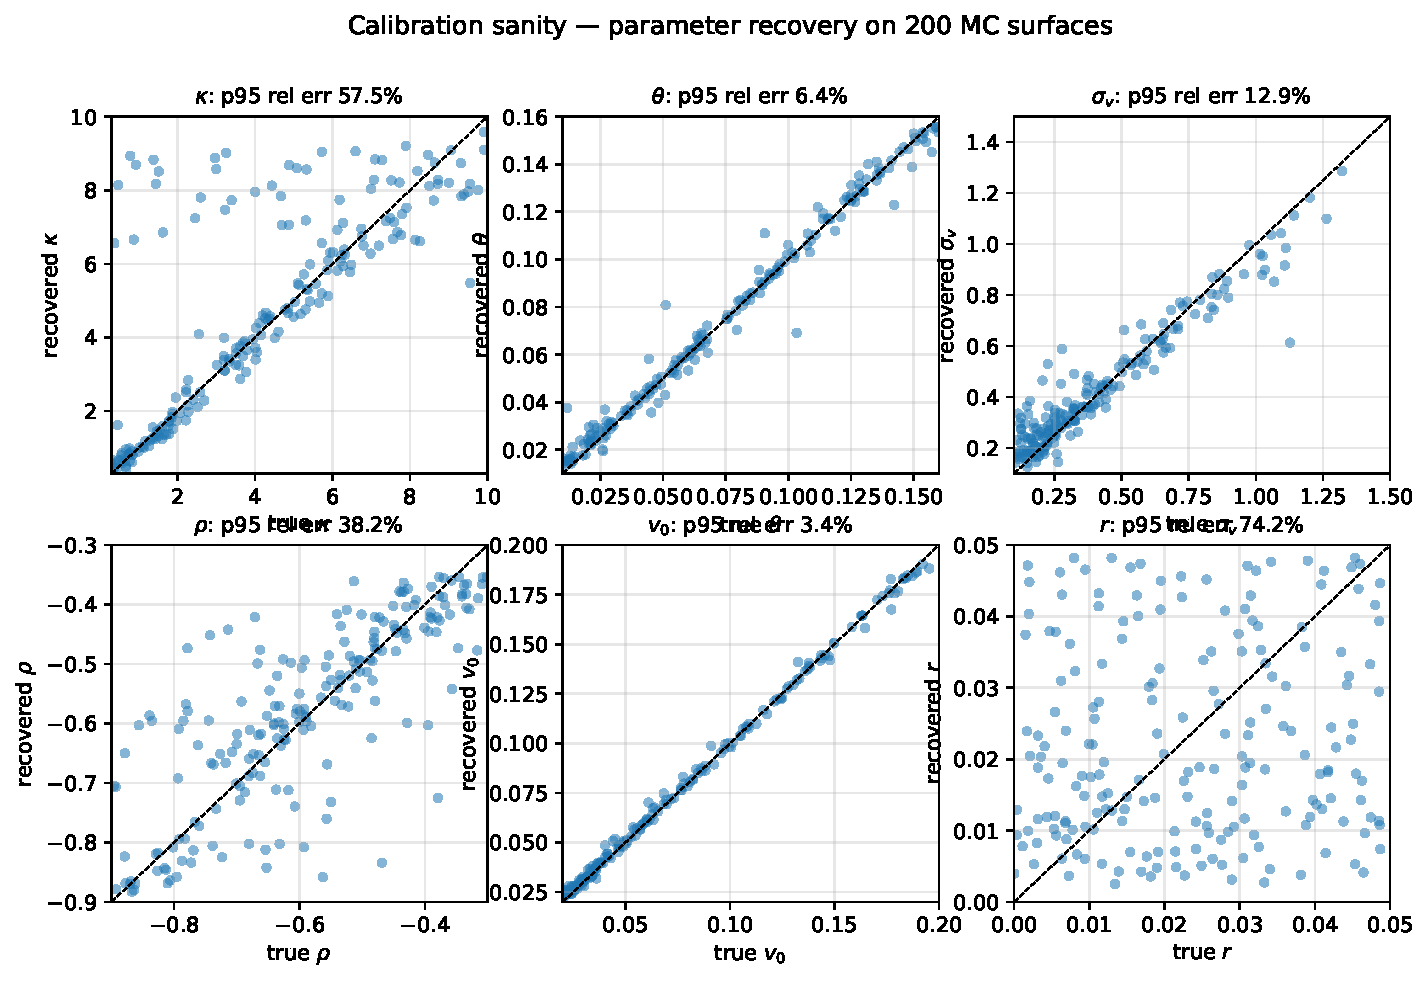
\includegraphics[width=\linewidth]{figures/calibration_recovery.pdf}
  \caption{Recovered versus true parameters on the $200$-surface MC
  reference after a flat-init Adam inversion of the surrogate. Dashed
  lines are the identity. Per-parameter $p_{95}$ relative errors are
  reported in the titles.}
  \label{fig:cal}
\end{figure}

\cref{tab:cal} and \cref{fig:cal} report the outcome. Two kinds of
parameters emerge:

\begin{table}[h]
  \centering
  \begin{tabular}{lcccc}
    \toprule
    Parameter & Range & Mean $|\Delta|$ & $p_{95}|\Delta|$ & $p_{95}$ rel \\
    \midrule
    $\kappa$    & $[0.30,10.0]$   & $1.014$ & $5.58$  & $57.5\%$ \\
    $\theta$    & $[0.01,0.16]$   & $0.003$ & $0.010$ & $\phantom{0}6.4\%$ \\
    $\sigma_v$  & $[0.10,1.50]$   & $0.060$ & $0.180$ & $12.9\%$ \\
    $\rho$      & $[-0.90,-0.30]$ & $0.068$ & $0.229$ & $38.2\%$ \\
    $v_0$       & $[0.02,0.20]$   & $0.002$ & $0.006$ & $\phantom{0}3.4\%$ \\
    $r$         & $[0.00,0.05]$   & $0.015$ & $0.037$ & $74.2\%$ \\
    \bottomrule
  \end{tabular}
  \caption{Parameter recovery error. $p_{95}$ relative is
  $p_{95}|\Delta|$ divided by the range width.}
  \label{tab:cal}
\end{table}

The \emph{well-identified} parameters $v_0, \theta, \sigma_v$ recover
with $p_{95}$ relative errors of $3.4\%,\,6.4\%,\,12.9\%$; these are
the quantities that actually dictate the short- and long-maturity
ATM levels and the convexity of the skew. The \emph{poorly-identified}
set $\kappa, \rho, r$ reflects the classical Heston identifiability
problem: the pair $(\kappa,\rho)$ trades off along the leverage
direction (a higher mean-reversion can be compensated by a more
negative correlation) and the rate $r$ is nearly degenerate with $v_0$
in the ATM region of a single-curve, flat-rate calibration. In
production calibration, $r$ would be fixed from the yield curve and
$\kappa$ regularised or constrained via a prior.

The post-fit per-surface IV-RMSE averages \SI{30.74}{\bps}
(median $\SI{25.82}{\bps}$, $p_{95}=\SI{70.11}{\bps}$) --- below the
surrogate's own flat-prior validation error on most surfaces,
confirming that the surrogate is smooth and invertible under
gradient descent.

\section{Discussion and future work}
\label{sec:discussion}

\subsection{What Scenario C establishes}

The pipeline produces a fully differentiable Heston IV surrogate whose
end-to-end error is dominated by a single-checkpoint training run of
$\sim\!25$ minutes on a single GPU; the MC gate evaluates consistency
against an independent SDE solver and the calibration sanity check
confirms the model is usable as a calibration target. The bug in
\cref{sec:ln-dropout-bug} is a reusable cautionary tale for any
architecture that mixes Dropout with downstream per-sample normalisation.

\subsection{What it does not yet achieve}

The $\SI{50}{\bps}$ gate misses the $95\%$ target by 5.4 percentage
points. Plausible remedies, ordered by expected return on effort:
\begin{enumerate}
  \item Deeper trunk ($N_B=10$--$12$) and/or wider head ($r=64$),
        with a proportionally longer training schedule.
  \item Focal re-weighting of the loss at the high-$p_{99}$ tails
        (short maturities, deep wings) once per-cell residuals are
        tracked.
  \item Independent loss on the pricable-region residual head only, to
        stop the grid head drifting on unpricable cells that leak into
        gradients during training.
\end{enumerate}
Concerning the calibration side, the three poorly-identified parameters
$\kappa,\rho,r$ are not a surrogate problem and would be handled at the
calibration layer by:
\begin{enumerate}
  \item fixing $r$ from the discount curve;
  \item imposing an informative prior on $\kappa$
        (e.g.\ log-normal centred at the historical mean-reversion);
  \item multi-start Adam from $\sim\!5$--$10$ seeds and keeping the
        lowest-RMSE minimum, which would dampen the $\kappa$-$\rho$
        tradeoff for well-conditioned surfaces.
\end{enumerate}

\subsection{Reproducibility}

All artefacts are checked into the repository:

\begin{tabular}{ll}
  \toprule
  \textbf{Artefact} & \textbf{Path} \\
  \midrule
  Trained checkpoint   & \texttt{runs/v2\_baseline/best.pt} \\
  Training log         & \texttt{runs/v2\_baseline/train\_log.csv} \\
  Training HDF5        & \texttt{data/heston\_pipeline\_v2.h5} \\
  Validation HDF5      & \texttt{data/heston\_pipeline\_v2\_val.h5} \\
  MC reference         & \texttt{data/heston\_mc\_reference.h5} \\
  MC-gate diagnostic   & \texttt{.../diagnostics/evaluate\_v2\_vs\_mc.py} \\
  Calibration sanity   & \texttt{.../diagnostics/calibrate\_sanity.py} \\
  Figure script        & \texttt{report/make\_figures.py} \\
  Results summary      & \texttt{SCENARIO\_C\_RESULTS.md} \\
  \bottomrule
\end{tabular}

\begin{thebibliography}{9}

\bibitem{heston1993}
S.~L.~Heston, \emph{A closed-form solution for options with stochastic
volatility with applications to bond and currency options},
Review of Financial Studies 6 (1993), 327--343.

\bibitem{albrecher2007little}
H.~Albrecher, P.~Mayer, W.~Schoutens, J.~Tistaert,
\emph{The little Heston trap},
Wilmott Magazine, January 2007, 83--92.

\bibitem{fangoosterlee2008}
F.~Fang, C.~W.~Oosterlee,
\emph{A novel pricing method for European options based on
  Fourier-cosine series expansions},
SIAM Journal on Scientific Computing 31 (2008), 826--848.

\bibitem{andersen2008simple}
L.~Andersen,
\emph{Simple and efficient simulation of the Heston stochastic
volatility model},
Journal of Computational Finance 11 (2008), 1--42.

\bibitem{durrleman2002}
V.~Durrleman,
\emph{From implied to spot volatilities},
PhD thesis, Princeton University (2004); see also
Finance and Stochastics 14 (2010) 157--177.

\end{thebibliography}

\end{document}
